
\begin{figure}[h]
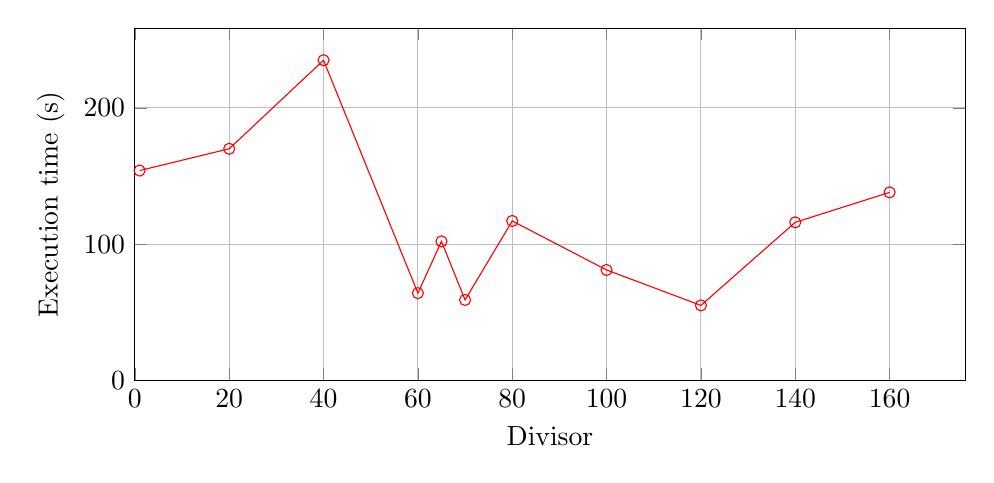
\begin{tikzpicture}
	\begin{axis}[width=\textwidth,height=40ex,xlabel=Divisor,ylabel=Execution time (s), xmin=0, ymin=0, grid=both]
	
	
	%% 5
\addplot[mark=o,color=red] coordinates {
(1,154)
(20,170)
(40,235)
(60,64)
(65,102)
(70,59)
(80,117)
(100,81)
(120,55)
(140,116)
(160,138)
};


\end{axis}

\end{tikzpicture}%
\caption{Example executions on the first instance. The search was first carried out systematically on every 20 values, then refined around what seemed to be a minimum, around 60-70.}
\end{figure}
